\documentclass{ximera}

\title{Introduction}
\author{Bart Snapp}

\begin{document}
\begin{abstract}
    What is Ximera?
\end{abstract}
\maketitle

Ximera, pronounced ``chimera,'' (\textbf{X}imera: \textbf{I}nteractive,
\textbf{M}athematics, \textbf{E}ducation,
\textbf{R}esources, for \textbf{A}ll) is an open-source platform that provides
tools for
authoring and publishing (PDF and Online), open-source, interactive educational
content, such as textbooks, assessments, and online courses.

\paragraph{Authors}  write and store their content on their own
machines and GitHub repositories.
Authors own their content and decide how to license their content. From a
single source written in \LaTeX, Ximera generates various output: PDF
worksheets,
PDF textbooks, and	PDF solution manuals, and so on. Of most interest,
Ximera can
also create online interactive activities:
\begin{center}
    \begin{tikzpicture}
        \node at (-1.8,.2)
        {\resizebox{.65cm}{!}{% \documentclass[tikz]{standalone}
% \makeatletter%%% to compile online
% \@ifundefined{bkgndcr}{
%   \usepackage{xcolor}
%   \colorlet{bkgndcr}{white}
%   \colorlet{txtcr}{black}
% }{}
% \makeatother  %%%
% \begin{document}
\begin{tikzpicture}[rounded corners=.5pt]
\draw[fill=bkgndcr] (0,0) -- (0,1.3) -- (.7,1.3) -- (1,1) -- (1,0) -- cycle;
\draw (.7,1.3) -- (.7,1) -- (1,1);
\end{tikzpicture}
% \end{document}}};
        \node at (-1.8,.2) {\small PDF};
        \node at (-2,0) {\resizebox{.65cm}{!}{% \documentclass[tikz]{standalone}
% \makeatletter%%% to compile online
% \@ifundefined{bkgndcr}{
%   \usepackage{xcolor}
%   \colorlet{bkgndcr}{white}
%   \colorlet{txtcr}{black}
% }{}
% \makeatother  %%%
% \begin{document}
\begin{tikzpicture}[rounded corners=.5pt]
\draw[fill=bkgndcr] (0,0) -- (0,1.3) -- (.7,1.3) -- (1,1) -- (1,0) -- cycle;
\draw (.7,1.3) -- (.7,1) -- (1,1);
\end{tikzpicture}
% \end{document}}};
        \node at (-2,0) {\small PDF};
        \node at (-2.2,-.2)
        {\resizebox{.65cm}{!}{% \documentclass[tikz]{standalone}
% \makeatletter%%% to compile online
% \@ifundefined{bkgndcr}{
%   \usepackage{xcolor}
%   \colorlet{bkgndcr}{white}
%   \colorlet{txtcr}{black}
% }{}
% \makeatother  %%%
% \begin{document}
\begin{tikzpicture}[rounded corners=.5pt]
\draw[fill=bkgndcr] (0,0) -- (0,1.3) -- (.7,1.3) -- (1,1) -- (1,0) -- cycle;
\draw (.7,1.3) -- (.7,1) -- (1,1);
\end{tikzpicture}
% \end{document}}};
        \node at (-2.2,-.2) {\small PDF};
        \draw[->] (-.6,0) -- (-1.4,0);
        \draw[->] (-.6,.2) -- (-1.4,.2);
        \draw[->] (-.6,-.2) -- (-1.4,-.2);
        \node at (0,0) {\resizebox{1cm}{!}{% \documentclass[tikz]{standalone}
% \makeatletter%%% to compile online
% \@ifundefined{bkgndcr}{
%   \usepackage{xcolor}
%   \colorlet{bkgndcr}{white}
%   \colorlet{txtcr}{black}
% }{}
% \makeatother  %%%
% \begin{document}
\begin{tikzpicture}[rounded corners=.5pt]
\draw[fill=bkgndcr] (0,0) -- (0,1.3) -- (.7,1.3) -- (1,1) -- (1,0) -- cycle;
\draw (.7,1.3) -- (.7,1) -- (1,1);
\end{tikzpicture}
% \end{document}}};
        \node at (0,0) {\LaTeX};
        \draw[->] (.6,0) -- (1.4,0);

        \node at (2,0) {\resizebox{1cm}{!}{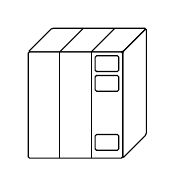
\begin{tikzpicture}[rounded corners=.5pt]
    \draw (0,0) rectangle (1.2,1.35);
    \draw (.4,0) -- (.4,1.35);
    \draw (.8,0) -- (.8,1.35);

    \draw (0,0)+(.85,1.1) rectangle ([shift={(.85, 1.1)}] .3, .2);
    \draw (0,0)+(.85,.85) rectangle ([shift={(.85, .85)}] .3, .2);
    \draw (0,0)+(.85,.1) rectangle ([shift={(.85, .1)}] .3, .2);

    \draw (1.2,0) -- (1.2,1.35) -- (1.5,1.65) -- (1.5,.3) -- cycle;

    \draw (0,1.35) -- (.3,1.65) -- (1.5,1.65) -- (1.2,1.35) -- cycle;
    \draw (.4,1.35) -- (.7,1.65);
    \draw (.8,1.35) -- (1.1,1.65);    
\end{tikzpicture}}};
        \draw[->] (2.6,0) -- (3.4,0);
        \node at (4,0) {\resizebox{1cm}{!}{\documentclass[tikz]{standalone}
\makeatletter%%% to compile online
\@ifundefined{bkgndcr}{
  \usepackage{xcolor}
  \colorlet{bkgndcr}{white}
  \colorlet{txtcr}{black}
}
\makeatother  %%%
\begin{document}
\begin{tikzpicture}[rounded corners=.1pt]
    \draw (-.15,-.1) rectangle (.95,.5);
    \draw[fill=bkgndcr] (0,0) rectangle (1,.8);
    \draw[fill=bkgndcr] (0,0) -- (-.2,.1) -- (-.2,.9) -- (.8,.9) -- (1,.8) -- (0,.8) --
    cycle;
    \draw (0,.8) -- (-.2,.9);
    \draw[fill=bkgndcr] (0,-.05) -- (1,-.05) -- (1,-.25) -- (0,-.25) -- cycle;
    \draw[fill=bkgndcr] (0,-.05) -- (0,-.25) -- (-.2,-.15) -- (-.2,.05) -- cycle;
    \draw[rounded corners=.5pt,fill=txtcr!50!bkgndcr] (.1,.1) rectangle  (.9,.7);
    \draw (-.2,-.25) -- (1.1,-.25) -- (1.2,-.37) -- (-.1,-.37) -- cycle;
    \draw (-.2,-.25) -- (-.2,-.3) -- (-.1,-.4) -- (-.1,-.37) -- cycle;
    \draw (-.1,-.4) rectangle (1.2,-.37);
\end{tikzpicture}
\end{document}}};
        \node at (-2,-1) {Various};
        \node at (-2,-1.4) {PDFs};
        \node at (0,-1) {Single};
        \node at (0,-1.4) {Source};
        \node at (2,-1) {Deploy};
        \node at (2,-1.4) {Server};
        \node at (4,-1) {Students};
        \node at (4,-1.4) {Engage};

    \end{tikzpicture}
\end{center}
The source code used to produce PDFs can also create interactive online
activities when deployed to a Ximera server. Students access this content via a
URL or an assignment in their LMS.

\paragraph{Get involved} by contributing as an instructor, author,
or developer. To get started with Ximera, visit our
\textit{First Steps in Ximera} GitHub repository:
\begin{center}
    \qrcode{\xfsURL}\\
    \small\url{\xfsURL}
\end{center}
\textbf{This document assumes you have completed the instructions there, and have
successively deployed Ximera content online.}

\paragraph{Funding for the Ximera Project} is provided by
a U.S.\ Department of Education Open Textbooks Pilot Program grant in the
amount of \$2,125,000, from 2024--2026, with no external funding.
In the past, the Ximera Project has
also received support from NSF Grant DUE-1245433, the Shuttleworth
Foundation, the Ohio State University
Department of Mathematics, and the Affordable Learning Exchange at OSU.


As a token of our appreciation, \textbf{consider applying for a Ximera
    Flash-Grant Stipend:}
\begin{center}
    \qrcode{\xfgURL}\\
    \small\url{\protect\xfgURL}
\end{center}
Thank you for your interest in Ximera. We encourage you to contact the
team with any questions you may have.
\end{document}
